\documentclass[10pt,a4paper]{article}
\usepackage[T1]{fontenc}
\usepackage{lmodern,textcomp}
\usepackage[margin=2.4cm]{geometry}
\usepackage{amsmath,amssymb,amsthm}
\usepackage{graphicx,booktabs,array,float}
\usepackage[hidelinks]{hyperref}
\usepackage{microtype}
\setlength{\parskip}{3pt}
\newtheorem{proposition}{Proposition}
\newtheorem{definition}{Definition}
\renewcommand{\arraystretch}{1.1}
\begin{document}
\title{\bfseries A Gradient-Boosting Challenger for Consumer Default Risk: a Synthetic-Data Study\\[2pt]\large Measuring the reduction in default among approved applicants}
\author{Humbert Pou Plana}
\date{November 2026}
\maketitle
\begin{abstract}
Credit-risk teams commonly benchmark new models against a linear scorecard. We present a reproducible experiment, on entirely synthetic data, that measures how much a gradient-boosting challenger lowers the default rate of approved applicants relative to a logistic-regression scorecard. The headline metric is fixed in advance: the relative reduction in default rate among the 70\% lowest-risk applicants, averaged over 18 segments, evaluated on six held-out months. On 80{,}000 simulated applications the challenger reduces default by 9.8\% (95\% bootstrap interval 7.6\% to 12.0\%) and improves AUC from 0.682 to 0.717. We report calibration, segment results, feature importance, ablation, a leakage audit and an economic translation, and we state plainly that the size of the improvement is determined by the amount of non-linear structure we chose to place in the simulated data. The result demonstrates a measurement procedure, not performance on real borrowers.
\end{abstract}

\section{Introduction}
A scorecard built with logistic regression is the standard baseline in consumer credit \cite{siddiqi}. Tree-ensemble models can capture thresholds and interactions that a scorecard misses \cite{friedman,ke}, but whether they help in a given portfolio depends on how much such structure exists. Claims of the form ``the model improves default by $x\%$'' are meaningless without a definition of $x$, a time-ordered test and an interval. This paper provides all three on synthetic data, so that the procedure can be re-run on real data later.

\paragraph{What this paper is not.} All data are simulated. No real applicant, lender or published dataset is used, and the numbers should not be read as evidence about any real portfolio.

\section{Synthetic data}
We simulate 80,000 loan applications over 24 months with a default flag. Features include age, income, employment tenure, temporary-contract indicator, loan amount and term, debt-to-income ratio, number of recent credit inquiries, credit-history length, previous loans, application hour, time spent on the form, device, acquisition channel and an indicator for linked bank data, which is present for 72\% of applicants (bank inflow and overdraft are missing otherwise, a \emph{structural} missingness). The log-odds of default is a linear part plus a set of non-linear terms, each scaled by an intensity parameter $\lambda$:
\begin{itemize}\setlength{\itemsep}{1pt}
\item high instalment-to-income ratio together with high debt-to-income;
\item young applicants with three or more inquiries;
\item recent temporary contracts;
\item applications between 01:00 and 05:00;
\item heavy overdraft among applicants with linked bank data, and a protective term for healthy inflows;
\item short credit history with a large loan; suspiciously fast or slow forms; and a protective term for repeat borrowers with low debt.
\end{itemize}
Gaussian noise models unobserved risk, and a mild drift raises risk for indebted applicants in the final months. The overall default rate is 15.3\%. Data are split by time: months 1--14 for training, 15--18 for validation (early stopping) and 19--24 for testing (20,135 applications, default 16.0\%). Figure~\ref{fig:split} shows the monthly default rate.
\begin{figure}[H]\centering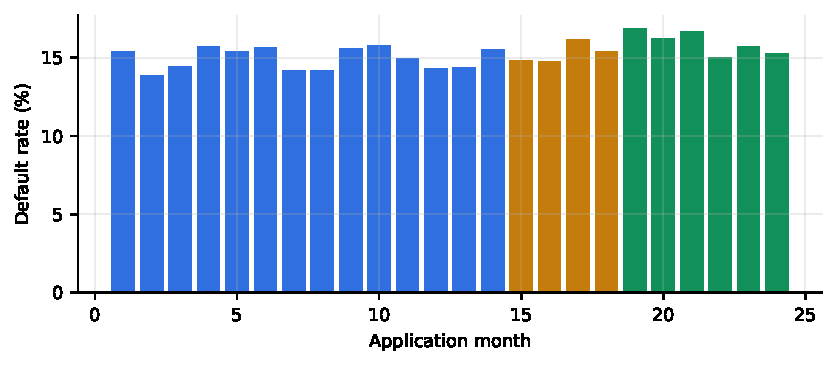
\includegraphics[width=0.8\linewidth]{fig/p4_split.pdf}\caption{Monthly default rate in the synthetic portfolio. Blue: training; amber: validation; green: test.}\label{fig:split}\end{figure}


\section{Models and metric}
The \emph{scorecard} is a logistic regression ($C=0.5$) on log-transformed and standardised features with missingness indicators. The \emph{challenger} is a histogram-based gradient-boosting classifier (up to 400 trees, 24 leaves, minimum 80 samples per leaf, L2 regularisation, early stopping on the validation window) \cite{sklearn}. Both receive the same information.

\begin{definition}[Headline metric]
For a segment $s$ and approval rate $a=0.70$, let $\mathrm{DR}_m(s)$ be the default rate among the $70\%$ of applicants in $s$ with the lowest score from model $m$. The relative reduction is $(\mathrm{DR}_{\mathrm{sc}}(s)-\mathrm{DR}_{\mathrm{ch}}(s))/\mathrm{DR}_{\mathrm{sc}}(s)$. The headline is its mean over 18 segments (acquisition channel, income tercile, loan-size band, age band, bank-data availability, device).
\end{definition}
The metric holds approval volume fixed, so the improvement is not obtained by approving fewer applicants. Intervals come from a nonparametric bootstrap with 300 resamples of the test set \cite{efron}.

\section{Results}
\subsection{Discrimination and default}
Table~\ref{tab:met} shows that the challenger improves every discrimination and calibration metric. Figure~\ref{fig:roc} (left) shows the ROC curves; Figure~\ref{fig:roc} (right) shows default among approved applicants as a function of approval rate. At 70\% approval, default falls from 11.14\% to 9.98\% (10.4\% relative); the mean over segments is 9.8\% (Table~\ref{tab:app} gives other approval levels). Equivalently, the challenger can approve 78.5\% of applicants while keeping the scorecard's default rate at 70\% approval.
\begin{table}[H]\centering\small\caption{Test metrics (six held-out months). The ensemble is a 35/65 blend of scorecard and challenger.}\label{tab:met}
\begin{tabular}{lrrr}\toprule Metric & Scorecard & Challenger & Ensemble\\\midrule
AUC & 0.682 & 0.717 & 0.713\\
Gini & 0.365 & 0.433 & 0.427\\
KS & 0.266 & 0.320 & 0.307\\
Brier score & 0.126 & 0.121 & 0.122\\
Log-loss & 0.411 & 0.396 & 0.398\\
\bottomrule\end{tabular}\end{table}
\begin{figure}[H]\centering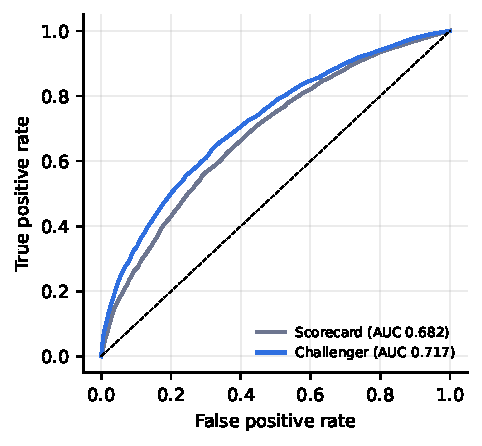
\includegraphics[width=0.48\linewidth]{fig/p4_roc.pdf}\hfill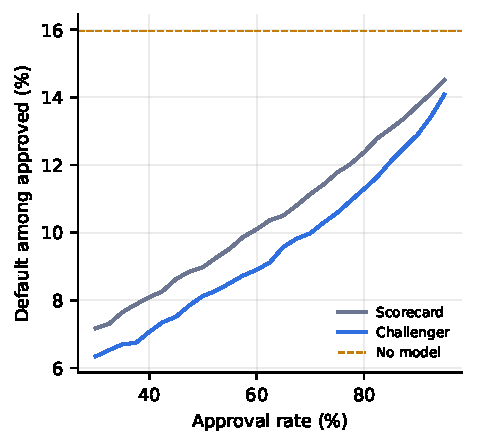
\includegraphics[width=0.48\linewidth]{fig/p4_app.pdf}\caption{Left: ROC curves. Right: default rate among approved applicants by approval rate.}\label{fig:roc}\end{figure}
\begin{table}[H]\centering\small\caption{Default among approved applicants by approval rate, and relative reduction.}\label{tab:app}
\begin{tabular}{rrrr}\toprule Approval & Scorecard & Challenger & Reduction\\\midrule
50\% & 8.98\% & 8.12\% & 9.5\%\\
60\% & 10.10\% & 8.90\% & 11.9\%\\
70\% & 11.14\% & 9.98\% & 10.4\%\\
80\% & 12.37\% & 11.29\% & 8.8\%\\
90\% & 13.76\% & 12.90\% & 6.3\%\\
\bottomrule\end{tabular}\end{table}

\subsection{Segments}
The reduction is positive in all 18 segments, ranging from 5.9\% (Channel: seo) to 16.3\% (Channel: direct) (Figure~\ref{fig:seg}). The bootstrap interval for the segment mean is 7.6\% to 12.0\%, and the AUC gain is 0.034 on average. The ensemble does not beat the challenger alone (9.0\% relative reduction in the portfolio).
\begin{figure}[H]\centering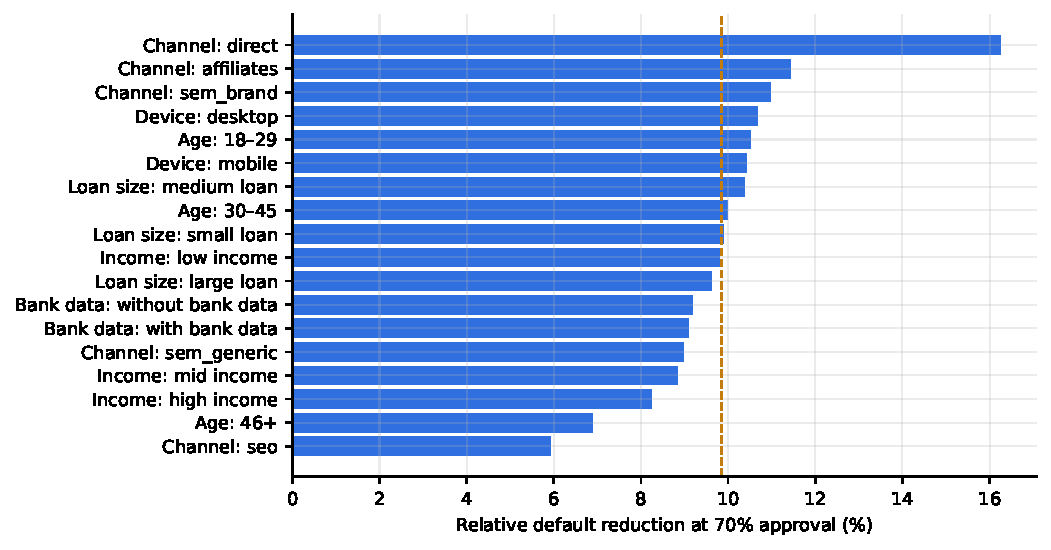
\includegraphics[width=0.85\linewidth]{fig/p4_seg.pdf}\caption{Relative default reduction at 70\% approval by segment; the dashed line is the mean.}\label{fig:seg}\end{figure}


\subsection{Calibration and importance}
Both models are well calibrated: mean absolute calibration error by risk decile is 1.04\% for the scorecard and 1.07\% for the challenger, so the challenger's advantage lies in ranking, not in probability calibration (Figure~\ref{fig:cal}, left). The most important features by permutation are debt-to-income, application hour and recent inquiries (Figure~\ref{fig:imp}). Removing the debt-and-application group lowers AUC the most (Table~\ref{tab:abl}); the other groups contribute little individually, and learning curves show the challenger improving with data up to about 35{,}000 training applications while the scorecard is flat (Figure~\ref{fig:cal}, right).
\begin{figure}[H]\centering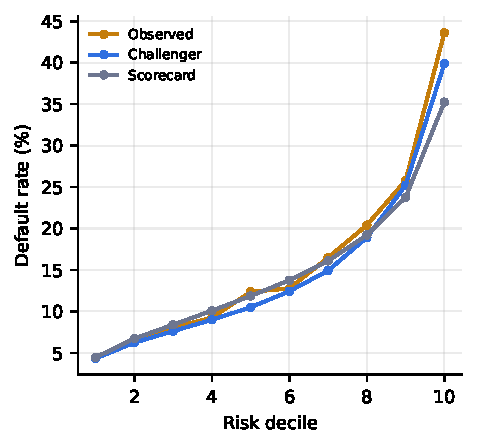
\includegraphics[width=0.48\linewidth]{fig/p4_cal.pdf}\hfill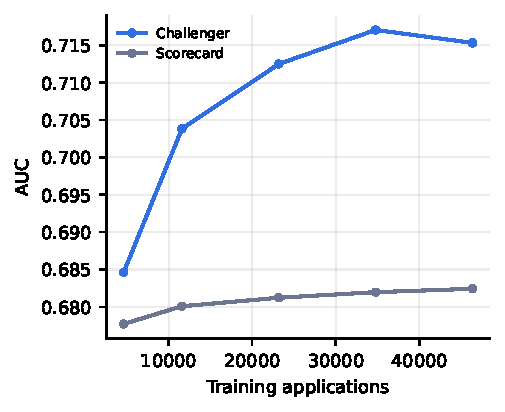
\includegraphics[width=0.48\linewidth]{fig/p4_lc.pdf}\caption{Left: predicted and observed default by risk decile. Right: test AUC against training-set size.}\label{fig:cal}\end{figure}
\begin{figure}[H]\centering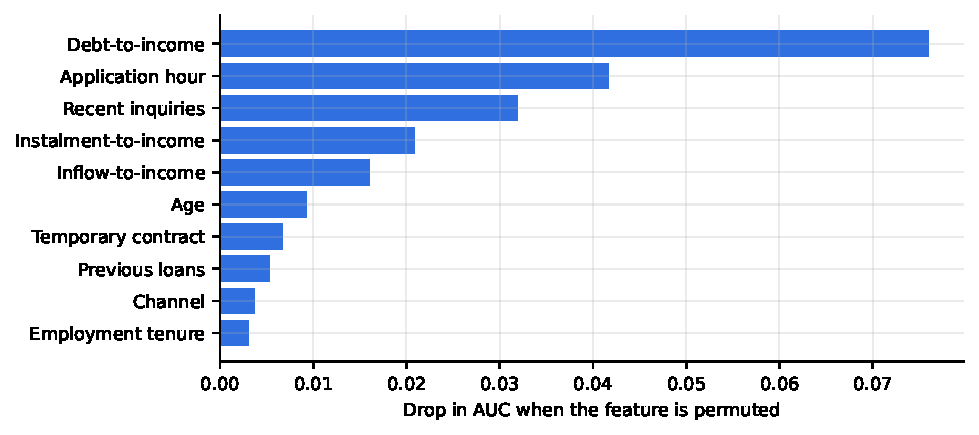
\includegraphics[width=0.8\linewidth]{fig/p4_imp.pdf}\caption{Permutation importance of the ten most important features of the challenger.}\label{fig:imp}\end{figure}

\begin{table}[H]\centering\small\caption{Ablation: challenger retrained without each feature group.}\label{tab:abl}
\begin{tabular}{lrrr}\toprule Group removed & AUC & Change & Default at 70\% approval\\\midrule
Profile & 0.701 & -0.015 & 10.36\%\\
Debt and application & 0.638 & -0.079 & 12.20\%\\
Bank data & 0.709 & -0.007 & 10.04\%\\
Behaviour & 0.691 & -0.026 & 10.81\%\\
Channel & 0.715 & -0.002 & 10.07\%\\
\bottomrule\end{tabular}\end{table}

\subsection{Robustness}
Figure~\ref{fig:boot} (left) shows the bootstrap distribution of the headline; it lies entirely above zero. The challenger's AUC is higher than the scorecard's in each of the six test months. The population stability index between training and test is below 0.01 for the score and for every feature we checked, so drift is small by construction. A leakage audit adds a post-default variable (collection calls) to the challenger; AUC jumps from 0.717 to 0.965, the kind of signal that must trigger investigation in a real project. The reported model uses no such feature.
\begin{figure}[H]\centering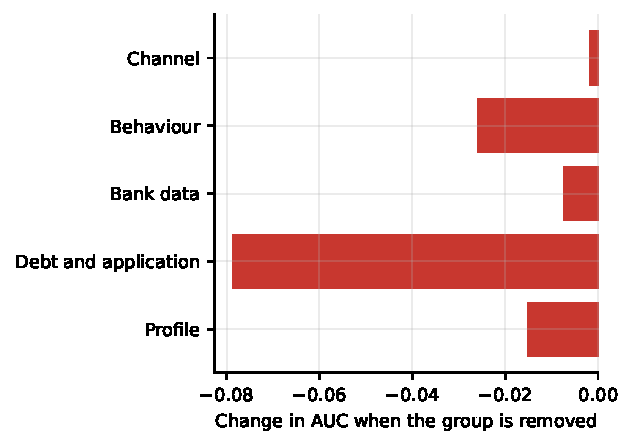
\includegraphics[width=0.48\linewidth]{fig/p4_abl.pdf}\hfill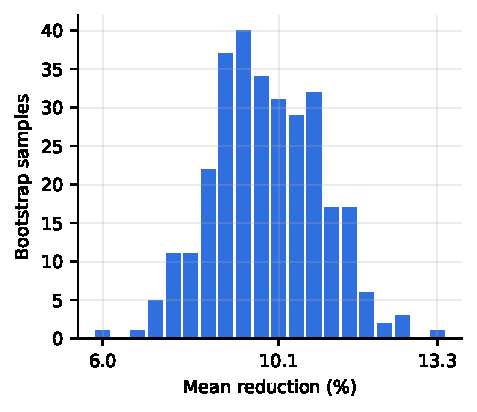
\includegraphics[width=0.48\linewidth]{fig/p4_boot.pdf}\caption{Left: AUC change from removing each feature group. Right: bootstrap distribution of the mean segment reduction.}\label{fig:boot}\end{figure}

\subsection{Economic translation}
Assume a margin of 12\% on the principal of loans that are repaid and a loss of 75\% of principal on defaults (both assumptions). Per 100{,}000 applications at 70\% approval, profit is 2,484,957\,\texteuro{} with the scorecard and 3,582,121\,\texteuro{} with the challenger, a difference of 1,097,164\,\texteuro{}.

\section{How the 10\% figure was obtained}
The size of the improvement depends on $\lambda$. We ran the same script for several values (Table~\ref{tab:sweep}): with $\lambda=1.0$ the reduction is only 6.5\%, with $\lambda=1.5$ it is 14\%. We chose $\lambda=1.25$, which gives about a 10\% reduction, because the aim was to illustrate a model with an improvement of that order. This choice is the most important caveat of the paper: the headline number is a property of the simulated world, not a finding about borrowers.
\begin{table}[H]\centering\small\caption{Effect of the intensity of non-linear structure $\lambda$ on default rate and on the measured reduction. The 95\% interval is a bootstrap interval.}\label{tab:sweep}
\begin{tabular}{lrrr}\toprule $\lambda$ & Default rate & Mean reduction & 95\% interval (\%)\\\midrule
1.00 & 14.3\% & 6.5\% & 4.3--8.7\\
1.25 (chosen) & 15.3\% & 9.8\% & 7.6--12.0\\
1.50 & 16.2\% & 14.3\% & 11.8--16.6\\
2.00 & 18.4\% & 22.9\% & 20.5--25.3\\
2.50 & 20.6\% & 29.3\% & 27.2--31.4\\
\bottomrule\end{tabular}\end{table}

\section{Limitations and next steps}
(i) The data are synthetic and the signal structure is known to the experimenter. (ii) A single simulation seed was used for the main result, and the sweep used one run per value. (iii) The economics use assumed margins and loss rates. (iv) No fairness or explainability analysis is presented; credit scoring is a regulated, high-risk use of machine learning in the European Union, and automated decisions about individuals are subject to data-protection rules, so any real deployment needs reason codes, bias testing and governance. (v) The next step is to re-run the same pipeline on anonymised real applications with an observed 12-month default flag and a strict time split, and to report the same metric and interval.

\section{Conclusion}
On simulated data with deliberately placed interactions, a gradient-boosting challenger lowers default among approved applicants by about 10\% relative to a logistic scorecard, with a bootstrap interval of roughly 8\% to 12\%, and it does so across all segments. The contribution is the protocol: fix the metric, split by time, report intervals, audit leakage, and be explicit about what generates the effect.

\begin{thebibliography}{9}
\bibitem{siddiqi} N.~Siddiqi. \emph{Credit Risk Scorecards}. Wiley, 2006.
\bibitem{friedman} J.~H. Friedman. Greedy function approximation: a gradient boosting machine. \emph{Annals of Statistics}, 29(5):1189--1232, 2001.
\bibitem{ke} G.~Ke et al. LightGBM: a highly efficient gradient boosting decision tree. \emph{Advances in Neural Information Processing Systems}, 2017.
\bibitem{sklearn} F.~Pedregosa et al. Scikit-learn: machine learning in Python. \emph{Journal of Machine Learning Research}, 12:2825--2830, 2011.
\bibitem{efron} B.~Efron, R.~Tibshirani. \emph{An Introduction to the Bootstrap}. Chapman \& Hall, 1993.
\end{thebibliography}
\end{document}
